\documentclass[a4paper,oneside]{memoir}
\usepackage[english]{babel}
\usepackage[T1]{fontenc}
\usepackage[utf8]{inputenc}
\usepackage{wallpaper}
\usepackage{palatino}
\usepackage{graphicx}
\usepackage{tikz}


\usepackage{xcolor,fix-cm}
\definecolor{numbercolor}{gray}{0.7}
\newif\ifchapternonum
\makechapterstyle{jenor}{
\renewcommand\printchaptername{}
\renewcommand\printchapternum{}
\renewcommand\printchapternonum{\chapternonumtrue}
\renewcommand\chaptitlefont{\fontfamily{pbk}\fontseries{db}%
\fontshape{n}\fontsize{25}{35}\selectfont\raggedleft}
\renewcommand\chapnumfont{\fontfamily{pbk}\fontseries{m}\fontshape{n}%
\fontsize{1in}{0in}\selectfont\color{numbercolor}}
\renewcommand\printchaptertitle[1]{%
\noindent%
\ifchapternonum%
\begin{tabularx}{\textwidth}{X}%
{\parbox[b]{\linewidth}{\chaptitlefont ##1}%
\vphantom{\raisebox{-15pt}{\chapnumfont 1}}}
\end{tabularx}%
\else
\begin{tabularx}{\textwidth}{Xl}
{\parbox[b]{\linewidth}{\chaptitlefont ##1}}
& \raisebox{-15pt}{\chapnumfont \thechapter}%
\end{tabularx}%
\fi
\par\vskip2mm\hrule
}
}

\usepackage{kpfonts}
\setSingleSpace{1.1}
\SingleSpacing
\usepackage{xcolor,calc}
\definecolor{chaptercolor}{gray}{0.8}
% helper macros
\newcommand\numlifter[1]{\raisebox{-2cm}[0pt][0pt]{\smash{#1}}}
\newcommand\numindent{\kern37pt}
\newlength\chaptertitleboxheight
\makechapterstyle{hansen}{
\renewcommand\printchaptername{\raggedleft}
\renewcommand\printchapternum{%
\begingroup%
\leavevmode%
\chapnumfont%
\strut%
\numlifter{\thechapter}%
\numindent%
\endgroup%
}
\renewcommand*{\printchapternonum}{%
\vphantom{\begingroup%
\leavevmode%
\chapnumfont%
\numlifter{\vphantom{9}}%
\numindent%
\endgroup}
\afterchapternum}
\setlength\midchapskip{0pt}
\setlength\beforechapskip{0.5\baselineskip}
\setlength{\afterchapskip}{3\baselineskip}
\renewcommand\chapnumfont{%
\fontsize{4cm}{0cm}%
\bfseries%
\sffamily%
\color{chaptercolor}%
}
\renewcommand\chaptitlefont{%
\normalfont%
\huge%
\bfseries%
\raggedleft%
}%
\settototalheight\chaptertitleboxheight{%
\parbox{\textwidth}{\chaptitlefont \strut bg\\bg\strut}}
\renewcommand\printchaptertitle[1]{%
\parbox[t][\chaptertitleboxheight][t]{\textwidth}{%
%\microtypesetup{protrusion=false}% add this if you use microtype
\chaptitlefont\strut ##1\strut}%
}
}


% \usepackage{titlesec, blindtext, color}
% \definecolor{gray75}{gray}{0.75}
% \newcommand{\hsp}{\hspace{20pt}}
% \titleformat{\chapter}[hang]{\Huge\bfseries}{\thechapter\hsp\textcolor{gray75}{|}\hsp}{0pt}{\Huge\bfseries}

% Setup captions
%\captionstyle[\centering]{\centering}
%\changecaptionwidth
%\captionwidth{0.8\linewidth}

% Protect against widows and orphans
%\clubpenalty=10000
%\widowpenalty=10000

%\linespread{1.2}

%\raggedbottom

% \chapterstyle{ger}
% \chapterstyle{ell}
% \chapterstyle{companion}
% \chapterstyle{hangnum}
% \chapterstyle{lyhne} % OKish
% \chapterstyle{madsen} % OK
% \chapterstyle{jenor} % Font too big
% \chapterstyle{wilsondob}
\chapterstyle{hansen} % OK

%\maxsecnumdepth{subsection}

%%  Setup fancy style quotation
%%  ==================================================================
%\usepackage{tikz}
%\usepackage{framed}

%\newcommand*\quotefont{\fontfamily{fxl}} % selects Libertine for quote font

% Make commands for the quotes
%\newcommand*{\openquote}{\tikz[remember picture,overlay,xshift=-15pt,yshift=-10pt]
%     \node (OQ) {\quotefont\fontsize{60}{60}\selectfont``};\kern0pt}
%\newcommand*{\closequote}{\tikz[remember picture,overlay,xshift=15pt,yshift=5pt]
%     \node (CQ) {\quotefont\fontsize{60}{60}\selectfont''};}

% select a colour for the shading
%\definecolor{shadecolor}{rgb}{1,1,1}

% wrap everything in its own environment
%\newenvironment{shadequote}%
%{\begin{snugshade}\begin{quote}\openquote}
%{\hfill\closequote\end{quote}\end{snugshade}}

%%  Begin document
%%  ==================================================================
\begin{document}

%%  Begin title page
%%  ==================================================================
    \thispagestyle{empty}
    \ULCornerWallPaper{1}{cover/nat-farve.pdf}
    \ULCornerWallPaper{1}{cover/nat-en.pdf}
    \begin{adjustwidth}{-3cm}{-1.5cm}
    \vspace*{-1cm}
    \textbf{\Huge Bachelor Thesis} \\
    \vspace*{2.5cm} \\
    \textbf{\Huge Cache optimizations in garbage collection} \\
    \vspace*{.1cm} \\
    {\huge Dynamically selecting cache-frindly object layouts} \\
    \begin{tabbing}
    % adjust the hspace below for the longest author name
    David Himmelstrup \hspace{1cm} \= \texttt{<vrs552@alumni.ku.dk>} \\
    \\[12cm]
    \textbf{\Large Supervisor} \\
    Fritz Henglein \> \texttt{<henglein@diku.dk>} \\
    \end{tabbing}
    \end{adjustwidth}
    \newpage
    \ClearWallPaper
%%  ==================================================================
%%  End title page

\chapter*{Abstract}

\newpage

\tableofcontents*

\chapter{Introduction}
High level, memory managed languages offer many productivity advantages because
developers don't have to worry about how objects are arranged in memory. However,
memory layout can hugely affect performance so the productivity advantages can
come with efficiency disadvantages. Much research has been done not only to
quantify this discrepancy but also to narrow the gap.

In this thesis I will be looking at the memory layout of semi-space garbage
collector in the context of a purely functional programming language.
I will implement two optimizations in the garbage collector and evaluate these
optimizations against the baseline.

\section{Jikes RVM vs. native}
*Why I use a native GC rather than the Jikes RVM (Research Virtual Machine)
to test my hypothesis even though a lot of other people use it.
Answer: Haskell has different allocation patterns than Java*

\section{Research Aims}
I have implemented a new semi-space garbage collector for a subset of the
Haskell programming language. This collector contains two novel optimizations
that modify how objects are arranged in memory. It is my hypothesis that these
two optimizations will improve how the garbage collector interacts with the
memory caches. As part of this work I want to answer the following questions:
\begin{itemize}
  \item Is the implementation unreasonably complicated? Some previously proposed
    systems have shown promise on a small scale but were too complicated to be
    used outside of academia.
  \item Are the optimizations beneficial and do the benefits outweigh the costs?
  \item Can the optimizations be ported to collectors used in industry?
\end{itemize}

\section{Thesis organization}
Chapter 2 goes over the current approaches to garbage collection, how people
have tried to solve the problem in the past, and provides details about
LHC which are required by the later chapters.
Chapter 3 describes the design and implementation of the main contribution of
this thesis.
Chapter 4 describes the design and implementation of a furhter optimization that
follows as a direct consequence of the technique detailed in chapter 3.
Chapter 5 evaluates these two new approaches against a baseline collector. This
evaluation looks at deterministic factors which are proxies for performance.
Chapter 6 concludes the work and presents possible future work.

\chapter{Background}
\section{Processors, memory and cache}

CPUs used to run at similar frequencies as main memory, allowing them to read
from memory at roughly the same speed that it could process the information.
Sometimes programs has to process larger data sets than could fit into memory
and parts of the data set would have to be swapped out of main memory and onto
a disk or tape. A lot of caching research from that time was focused on how to
manage the virtual memory using limited physical memory (which supports direct
access with a constant latency) and a spinning disk drive (which requires seeking).

In recent years CPUs have gotten a lot faster, the bandwidth of memory
hasn't been able to keep pace and the memory latency has even gotten worse. This
means that fetching data from memory can easily be the bottleneck when processing
a data set. To solve this, several levels of memory caches were inserted closer
to the CPU. These caches work in levels with the lowest levels being smallest
and fastest. The caches have latencies that are roughly 100x to 10x quicker
than main memory. The caches also have higher bandwidth than main memory but
the benefit is less extreme here.

The introduction of caches meant that memory fetches no longer completed in a
constant amount of time because of the difference between a cache hit and
a cache miss. Just as seen with spinning disks earlier, certain access patterns
and data layouts can significantly improve performance. The canonical problems
that highlights this is matrix multiplication: The elements of the resulting
matrix can be computed in any order but choosing a cache-friendly access pattern
can be orders of magnitude faster.

% Write about MESI and cache associativity

\section{Manual memory management}
Still widely used in low-level languages and on embedded systems.
The onus is on the user to ensure correct usage.
Modern languages are usually garbage collected (8/10 most popular langauges on
github in 2017 were garbage collected).
Manual management has low overhead and can finalize objects immediately when
they're no longer used. This is important for limited resources such as file
handlers, file locks, etc.
Manual management often has more predictable performance without arbitrary pauses
but performs less well in terms of throughput and locality.

\section{Reference counting}
\section{Mark-and-sweep}
Unlike manual management and reference counting which never scans through all
the heap allocated objects, tracing garbage collection involves finding all live
heap objects by following a root set of objects out through all their children
and children's children. Once all the live objects have been found, unused memory
and resources can be reclaimed.
The mark-and-sweep does exactly this in two phases: First all objects reachable
from the root set are marked, then the "sweep" phases reclaims unused memory and
releases unused OS resources.
This algorithm correctly reclaims cyclic data structures when they're no longer
referenced but, similarly to manual management and reference counting, leads to
fragmentation and thus poor cache performance.

\section{Copying collectors}
In 1969, Fenichel et al published an algorithm for copying the reachable objects
into newly allocated memory chunk rather than merely marking them. Once the copying
is complete, all previously used memory will no longer contain live objects
and can be reclaimed. This makes the "sweep" phases unnecessary and it gets rid
of any fragmentation at the cost of requiring 2x available memory. The published
algorithm used stack space to traverse and copy the heap objects which is
undesirable since the stack space is limited and garbage collection will therefore
fail if the heap grows too large. One year later, Cheney published a non-recursive
algorithm for copying live objects and this algorithm has become the foundation
for essentially all modern copying garbage collectors. Since the algorithm is
non-recursive, it uses no stack space and works on heaps at any size.

Cheney's and Fenichel's algorithms both solve the same problem of copying a graph
with Cheney's algorithm having the decisive advantage of working on graphs of
unlimited size. However, the two algorithms also differ in the fact that Fenichel
copyed the graph in depth-first order and Cheney copies using breadth-first. This
different copy order affects cache performance but the effects wasn't too pronounced
with the architecture at the time and it wasn't unless 1984 that Moon et al
investigated the effect copy order has with virtual memory. And it wasn't until
1995 that the effects of copy order was quantified in relationship to the
CPU memory cache hierarchy by Nakashima and Chikayama.

Moon modified Cheney's algorithm to have two scanning pointers instead of one.
The to-space is divided up into blocks and the second scanning pointer always
points at the same block as the free pointer. Since objects are read (scavenged)
from the scanning pointer and children are copied (evacuated) to the free pointer,
this means the algorithm often only touches a single block even when the graph
is large and the free pointer is many blocks away from the first scanning pointer.
Since this is optimizing for block/page access, it can perform better when memory
is limited and page faults are expensive.

Moon's algorithm was later improved by Wilson, Lam, and Moher to reduce the
number of objects that are scavanged twice (scavanging is idempotent). Siegwart
and Hirzel further improved performance by adapting the algorithm for
multi-processor machines. Both groups of authors focused primarily on reducing
cache and TLB misses.

\section{Generational collectors}
It was found imperically that most allocated objects become unreachable (die)
almost immediately and that very few objects live for a significant fraction
of a programs total run-time. This effect of high infant mortality is exploited
by generational collectors by splitting the heap into two or more separate areas
(aka generations) that can be collected independently. A common configuration is
to have a minor and a major generation: New objects are allocated into the minor
generation and promoted into the major generation if they survive a collection.
Since it's relatively rare for older objects to contain pointers to younger
objects, only a small amount of bookkeeping is necessary to collect the minor
generation without tracing through all the live objects in the major generation.
In other words, infant objects can be allocated and collected without tracing or
copying long lived objects. This approach has proved so successful that, even
though the exact rate of infant mortality and object longevity varies from
program to program, generational GC is the default in most popular garbage
collected languages.

\section{Region inference}


\section{Haskell}
\section{GHC}
\section{LHC}
\section{Related work}
\subsection{Depth-first copying (two approaches)}
\subsection{immix}
\subsection{custom object layout (java)}

\chapter{Implementation}
\section{Tail-first copy order}

\section{Tail-pointer elimination}

\chapter{Evaluation}

\chapter{Conclusion}

% \chapter{Structure}
% \begin{enumerate}
%   \item Context (20\%): Motivate the problem (introduction, why should the reader care,
%     what have other people done)
%   \item Gap (10\%): Give the problem definition and what is missing from the current solutions
%   \item Innovation (50\%): Give the key-idea/detailed methods/experiemnts and evaluation (in that order)
%   \item (20\%) Talk about shortcomings of your approach, and future work, i.e. the conclusion.
% \end{enumerate}
%
% Context:
% \begin{enumerate}
%   \item Sequential access is faster (due to cache)
%   \item Breadth-first GC leads to non-sequential access
%   \item People have tried to solve it with hierarchical copying
%   \item Sequential data allows for pointers to be omitted
% \end{enumerate}
%
% Gap:
% \begin{enumerate}
%   \item Copying GC
%   \item Cheney's algorithm (zero stack, breadth-first ordering)
%   \item Depth-first ordering
%   \item Hierarchical ordering
% \end{enumerate}
%
% Innovation:
% \begin{enumerate}
%   \item Mixed depth-first/breadth-first ordering
%   \item Histogram of distances from parent to children.
%   \item Tail-pointer elimination
% \end{enumerate}
%
%
% \chapter{Introduction}
% Context (20\%): Motivate the problem (introduction, why should the reader care,
% what have other people done)
%
% Motivate the problem: CPUs have gotten a lot faster than memory and caches have been
% the answer, many modern languages use GC and copying can lead to better locality, locality is
% important, copying GC can have better locality than mark-and-sweep,
% describe cheney's algorithm, cheney not cache friendly because breadth-first,
% some tried to solve it by doing depth-first, other's by hierarchical order, immix
% (mixing copying and mark-sweep)
% Changing data layouts can lead to big performance improvements (50\% fewer misses, 20\%
% increased throughput)
%
% {section} cheney's algorithm is widely used but not very cache friendly.
%
% What does that reader need to know? GC, Semi-space GC, mark-and-sweep, cache
% behavior.
%
% Why should the reader care? Cheney algorithm is not cache friendly. Cache friendly
% access can be much faster.
%
% What have other people done? Depth-first copying, hierarchical copying, immix.
%
% \chapter{Gap}
% Give the problem definition and what is missing from the current solutions

\chapter{Tikz}
Tikz trial:

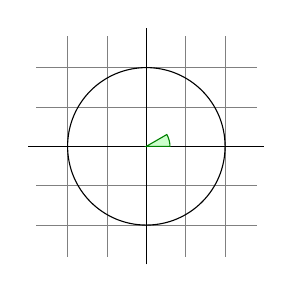
\begin{tikzpicture}
  \draw[step=.5cm,gray,very thin] (-1.4,-1.4) grid (1.4,1.4);
  \draw (-1.5,0) -- (1.5,0);
  \draw (0,-1.5) -- (0,1.5);
  \draw (0,0) circle [radius=1cm];
  \fill[green!20!white, draw=green!50!black] (0,0) -- (3mm,0mm)
    arc [start angle=0, end angle=30, radius=3mm] -- cycle;
\end{tikzpicture}


\end{document}
%%  ==================================================================
%%  End document
